\chapter{Introduction}
According to the Reuters Institute, 39\% of French adults use social media as a source of news in 2020.\footnote{\url{https://reutersinstitute.politics.ox.ac.uk/sites/default/files/2020-06/DNR_2020_FINAL.pdf}}  This share has declined since 2019, but this is mostly due to a decrease in the use of Facebook, while other networks are stable (like Twitter) or growing rapidly. This evolution of news consumption may reflect a growing appetite for stories that are not usually covered by traditional news media, or are covered in a different way.


In response to the transformation of news consumption, one should expect a change in the production of news by traditional media outlets. \citet{mcgregor_twitter_2018} find that journalists using Twitter as part of their daily work consider tweets to be as newsworthy as headlines from the Associated Press. Does this perception have an effect on the type of stories they choose to report? Does the success of a story on social media impact the news production by traditional news media outlets?

\section{Objective}

In this thesis, we seek to investigate the role of Twitter in the evolution of news production in recent years. Our objective is to find out to what extent events trending on social networks are  relayed more by traditional media outlets. The challenge is to precisely quantify and analyze the relationships between the two spheres, in a context of very strong co-dependence of each sphere.

Indeed, stories trending on Twitter always emerge in a context that fosters their propagation, and traditional news media are not isolated from that same context. For example, in the summer of 2018, far-left MP Jean-Luc Mélenchon called for a boycott of French President Emmanuel Macron's speech at the Palace of Versailles by spreading the hashtag \#MacronMonarc with other members of his party. Sympathizers were invited to tweet massively on the subject using this hashtag. That strategy was a major success on Twitter, as illustrated in Figure \ref{fig:macronmonarc}, and many traditional media outlets covered the boycott or mentioned the hashtag when reporting on the speech by the French President. However, one cannot state with certainty that the success of the online hashtag resulted in more articles on the boycott than Jean-Luc Mélenchon's statements alone would have done. At that time, Emmanuel Macron's popularity had dropped to its lowest level since the spring of 2017, and the statements made by his political opponent were closely watched by the media. Hence, the same context that favoured the success of the \#MacronMonarc hashtag may have prompted the coverage by mainstream media, without Twitter having any real effect. 

For an individual event, it is therefore impossible to disentangle the effects of the context, the intrinsic interest of the news, and the popularity on Twitter, in the choices made by news editors. However, the problem can be approached at an aggregate level: if we dispose of all the events covered both on Twitter and in the media, it is possible to highlight a systematic effect of popularity on Twitter. 

This is the approach we take in this thesis: we build a completely
new dataset including around 70\% of all the tweets in French during one year (July 2018 - July 2019) and the content produced online by the French-speaking general information media outlets during the same time period. We develop algorithms capable of grouping together tweets and news articles related to the same events. Finally, we study whether an event popularity on Twitter impacts the coverage that mainstream media devote to this event.

\begin{figure}
    \begin{subfigure}{1\textwidth}
 	    %\centering
        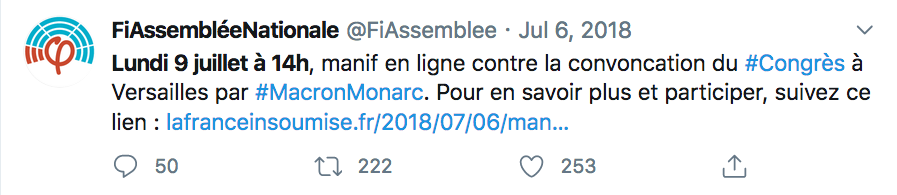
\includegraphics[width=1\textwidth]{figures/Beatrice/FirstTweetMacronMonarc.png}
        %\caption{2 seeds with an equal number of followers...}
        \label{fig:first_tweet_macronmonarc}
    \end{subfigure}
    \begin{subfigure}{1\textwidth}
 	    %\centering
        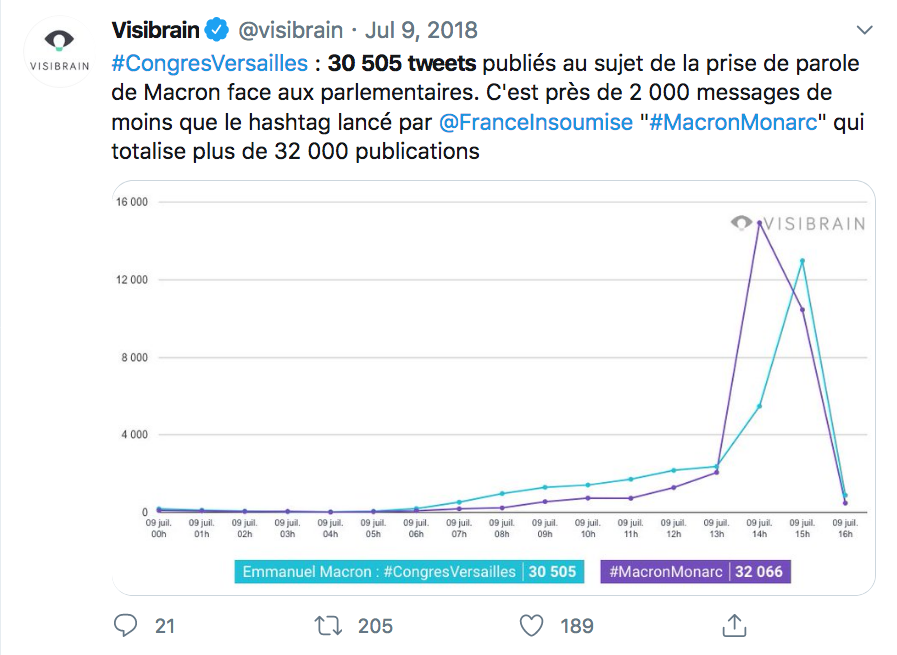
\includegraphics[width=1\textwidth]{figures/Beatrice/LastTweetMacronMonarc.png}
        %\caption{2 seeds with an equal number of followers...}
        \label{fig:last_tweet_macronmonarc}
    \end{subfigure}
    %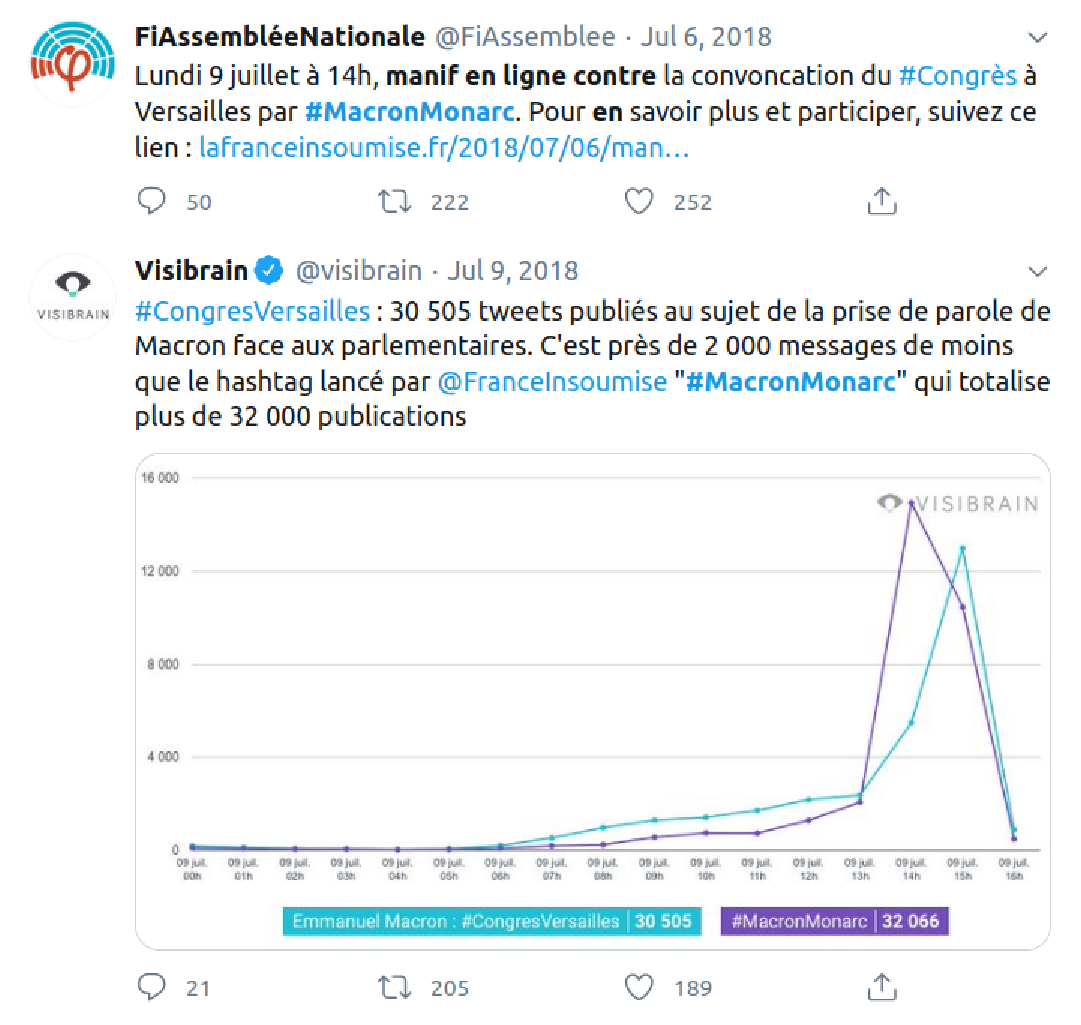
\includegraphics[width=.8\textwidth]{figures/Beatrice/MacronMonarc.pdf}
    \caption[Two tweets outlining the propagation history of the hashtag \#MacronMonarc]{Two tweets outlining the propagation history of the hashtag \#MacronMonarc. The upper tweet calls for an online protest against the speech of President Macron at the Palace of Versailles. The bottom tweet, published 3 days later, reports on the success of the \#MacronMonarc hashtag, compared to the other hashtag used to refer to the speech of Emmanuel Macron.}
    \label{fig:macronmonarc}
\end{figure}


The originality of this project is its multidisciplinary nature. On the one hand, it consists of an analysis in media economics, in order to determine causal factors that influence the success of news stories. On the other hand, drawing conclusions on all media events over the course of a year, as we propose to do, requires contributions in computer sciences involving the design of novel approaches for tweet collection, event detection and multimodal analysis. 
%The two disciplines, computer science and economics, do not have the same approaches, if only in the format expected of a thesis. Some chapters of this thesis will therefore be more accessible to researchers in computer science, and others more readable by economists.


\section{Scope of the study}
\subsubsection{Choice of Twitter}
%Why choose Twitter over another social network? Twitter is a micro-blogging website where users can post short messages named ``tweets". Tweets are limited to 280 characters, but can also contain pictures or videos. It is difficult to find reliable statistics on the number of tweets emitted every day worldwide. In 2014, Twitter announced the figure of 500 million tweets on average per day\footnote{\url{https://blog.twitter.com/official/en_us/a/2014/the-2014-yearontwitter.html}}, but there has been no other official statement since.   Several types of interactions are possible on this social network: users can ``follow" other users (that is to say, subscribe to their account in order to see all the tweets they publish), they can ``retweet" a tweet (re-publish it on their own account), ``reply" to it, ``quote" it (re-publish the tweet with a comment of their own) or ``like" it. Users can refer to other users in their tweets using ``mentions" (the user's handle preceded by "@"), and they can tag specific words as important using ``hashtags" (words preceded by ``\#"). Tweets are publicly visible by default, which is why Twitter is used by many public personalities like politicians or journalists. This is one of the main differences between Twitter and Facebook, where posts can by default only be read by one's ``friends" (usually people that one know in real life).

	
	Twitter is not the most used social network in France. According to the Reuters Intitute, in 2020 it is even the 4th French social network used for the consumption of news (used by 9\% of respondents), behind Facebook (43\%), YouTube (23\%) and Facebook Messenger (12\%). Nevertheless, we chose this network for our analysis of the relationships between social networks and traditional news media for several reasons. 

	
	First of all, \textbf{the structure of Twitter makes it a privileged tool for sharing news content}. Indeed, it favors public statements rather than private messages to family and friends, and encourages the sharing of external content (reference to other pages through URLs) because of the brevity of tweets. \citet{kwak_twitter_2010} even argue that the structure of Twitter makes it similar to a news media.
	
	
	Secondly, \textbf{Twitter has quickly become the preferred network of journalists}, who use it both to easily contact sources and to build a connection with their audience \citep{swasy_little_2016}. In the sample of journalists studied by \citet{mcgregor_twitter_2018}, 93\% had a Twitter account. A report conducted at the request of the European Commission\footnote{\url{http://ec.europa.eu/commfrontoffice/publicopinion/archives/quali/journsm_en.pdf}} shows a similar trend in Europe: the interviewed journalists make the distinction between Twitter, mostly used for work, and Facebook, more used in private life.
	
	
	Finally, \textbf{Twitter provides a larger access to its data than other social media platforms}. Even if the volume of tweets that one can access through Twitter's APIs is limited, the company still provides a free access to a rather large volume of data. Conversely, it is still nearly
impossible for researchers outside Facebook to get access to information on users' activity on the platform, with the exception of partnerships with a few rare research teams.

\subsubsection{Use of French tweets}

This thesis is part of the OTMedia project \citep{herve2019otmedia}, a platform for collecting and analysing French media developed at the Institut National de l'Audiovisuel (INA), the French media institute. This project aims to collect all contents published by French media online, regardless of their offline support (TV, radio, press, pure online media and press agencies). Therefore, the objective of the thesis was from the outset to work on the French media and their relationship with social networks, which meant collecting data from the French Twitter. However, it is quite difficult to know the country of Twitter users. On Twitter, there are two different ways to identify the location: through the location of the user and through the location of the tweet. 

First, users can indicate their location in their profile: nearly two third of the users in our sample do so. While the provided information is most often an actual location (e.g. ``Paris, France" or ``Val-d'Oise, Ile-de-France"), many users fill in this field with whimsical content (e.g. some users indicate ``Gotham City" or ``Everywhere and nowhere"). Nonetheless, we parsed this field for all authors of tweets in French in our sample, and, using OpenStreetMap, we associated each user to a country. Out of the $2,693,307$ users for which the location field is filled, the information provided allowed us to recover the country where the user is located in $72\%$ of the cases. $47\%$ of these users indicate that they are located in France.

Second, users can share their location at the time of their tweet. They can either decide occasionally to assign a location to their tweet, and are then presented a list of places, or they can decide to ``geo-tag" automatically all of their tweets. However, out of our $4,222,734 $ unique users, only $62,037$ (i.e. $1.5\%$) share their location in the first of their tweets we observe, and even less users ``geo-tag" their tweets: only $ 13,382$ (i.e. $0.32\%$) do so the first time we observe them, and $13,529$ the last time.

In both cases, filtering French tweets according to their location (or the location of their author) is likely to introduce biases or errors in our sample: on the one hand, the use of Open Street Map probably produces some false results (but we are not able to evaluate how many), and on the other hand, we do not know the factors that drive a user to share their location. They may be correlated with news consumption, for example.

We finally decided to work on all tweets in French, using the language metadata automatically determined by Twitter, without making assumptions about the country. This study has therefore gradually become a work on media production in French-speaking countries, since we have also extended the OTMedia collection to some  non-French (but French-speaking) media. The list of all collected media is presented in the \hyperlink{ref:Appendix}{Appendix}, in Section \ref{Sec:OA_Content}.

The choices we have made regarding the scope of this study lead in practice to a number of constraints, which we detail in the next section.

\section{Empirical challenges}

\subsubsection{Characterization of events}
According to the historian Pierre Nora, the emergence of the mass media has transformed the nature of events: \textit{``Press, radio, images are not only means from which events would be relatively independent, they are the very condition of their existence."}\footnote{``Presse, radio, images, n'agissent pas seulement comme des moyens dont les événements seraient relativement indépendants, mais comme la condition même de leur existence."}\citep{nora_evenement_1972}. The sociologist Patrick Champagne \citep{champagne_evenement_2000} shares the same view (\textit{``The media build the events they report"}\footnote{``les médias construisent les événements dont ils rendent compte"}) but highlights the fact that creating an event is a collective process: one media outlet alone cannot make the news if it is not picked up by others. A media event has thus to be reported by several sources to be defined as such.

With the appearance of social media, a new dimension has emerged: traditional news media cannot ignore a topic that is really bursting on Facebook or Twitter. In practice, many news events start nowadays on social media.  Social events and media events tend to be the same in many cases, that is what we call \textit{joint events}. However, any conversation or trend on social media cannot be considered as an event, but we lack an objective criterion that would allow us to distinguish between the everyday conversation and what constitutes an event on Twitter. Empirically we solve this problem by using the event definition proposed by \cite{mcminn_building_2013}:

“\textit{Definition 1.} An \textit{event} is a significant thing that happens
at some specific time and place.”

“\textit{Definition 2.} Something is \textit{significant} if it may be discussed in the media.”

With this definition in mind, we consider that any group of tweets that deal with the same subject can be considered as an event, but in practice we only consider joint events in the end, i.e. those that reach traditional media. The main challenge of this thesis in terms of machine learning is the design of a method to optimally detect joint events.

Another issue frequently raised when addressing the notion of event is that of granularity. Indeed, most events can be broken down into sub-events. For example, in a sports tournament, each match can be considered as a separate event, or the tournament itself can be considered as the event. From the point of view of computer science, this question can be reduced to a threshold issue: a low threshold will lead to the detection of small, very homogeneous events, while a higher threshold will lead to the formation of more general events. Choosing a particular threshold will not fundamentally change the validity of our study, as long as some variability in the choice of a threshold does not change our final results.

\subsubsection{Working on French tweets}
A common empirical challenge for researchers
using Twitter data comes from the fact that, because of the limits of the Twitter streaming APIs, one can only collect 1\% of the global volume of tweets at a given moment. Perhaps paradoxically, collecting tweets in a language with few speakers compared to English, Japanese or Spanish, that are the three most spoken languages on Twitter -- see Figure \ref{Figure:HistogramLanguagesFilter} -- becomes here an advantage. Indeed, with French tweets, we seek to collect only 1.8\% of all tweets sent worldwide, which seems an attainable target using several API access keys.

However, using a dataset of French tweets and news contents is also a challenge due to the still little amount of available corpora for Natural Language Processing and tweet analysis compared to English. We thus had to manually annotate our own event detection dataset, since the only other existing corpus for this task is in English. Besides, recent machine learning models handling text need to be pre-trained on massive datasets containing hundreds of thousands of examples. Tackling French-language documents, rather than English or Chinese, therefore means that the performance of the existing models will never be at the same level as the results described in the international machine learning literature.

\subsubsection{Including visual contents}
Communication on social networks is increasingly carried by visual supports (image, video or animated GIF). Recently, with the success of deep-learning based approaches and their ability to learn useful data representations \citep{bengio2013representation}, various approaches have been proposed for the learning of multimodal representation with an application to tasks such as Image Captioning, Visual Question Answering or Cross-Modal Image-Text Retrieval. These tasks suppose to learn from image-text pairs that are aligned: the text is a description of the picture, or the image is an illustration of the text. Under this condition, it is possible to learn a common representation of text and image in the same latent space. However, the text-image relationship on Twitter is rarely of this nature. For example, memes\footnote{A meme is an amusing image or video that spreads virally on the Internet, often with slight variations. See Figure \ref{Figure:meme} for a classical example of meme.} are quite different from illustrations: the same meme image is reused thousands of times in different contexts, associated with a text that gives it a different meaning.

In this thesis, we attempt to address the problem of multimodal representation of tweets by forming joint representations of text and image. However, we do not obtain representations that outperform text alone for the task of event detection.

\subsubsection{Collecting representative data}

By opting for a multidisciplinary thesis, which combines the prerequisites of econometrics with those of machine learning, we set ourselves additional criteria for the quality of our data. In machine learning, a biased dataset is defined relatively to a specific task: a bias in a dataset built to learn a specific task will lead to false conclusions when trying to solve the same task on different data (see for example \citep{tommasi2017deeper}).

However, in order to obtain valid conclusions in econometrics, the definition of bias must be stricter: an unbiased dataset is a subset of the overall population that is being described that proportionally reflects all the characteristics of that population. Here, if we can consider that our collection of media content reaches virtually the entire universe of French articles, we had to design a method of collecting tweets that would guarantee the absence of bias in tweets. To achieve this, we used as a reference the tweets feed provided by Twitter's Sample API, which provides a random sample of tweets emitted at a given time.

Another key issue here is data completeness: since the author of the first tweet of an event is a critical element for our final conclusions (we are particularly interested in its centrality in the Twitter network), it is important that we capture the actual first tweet of each event, not the second or third. Ideally, this means capturing the complete corpus of all tweets published in French. According to our estimates, our collection method yields between 74 and 78\% of the original tweets (i.e. not the retweets), thus guaranteeing the completeness of the data in the vast majority of events.

\subsubsection{Designing scalable methods}
Finally, as our constraints in terms of completeness led us to collect about 5 million tweets per day for one year, for a final corpus of 1.8 billion tweets, our event detection methods must necessarily be extremely time and memory efficient. One way to speed up processing was to work only on the original tweets (37\% of tweets), and to aggregate the retweets a posteriori into events. However, the speed of algorithms remains a central concern of our work. 

\section{Detailed Outline}
In order to solve the set of empirical challenges detailed in the previous section, the thesis is organized as follows.

The first step (see Chapter \ref{Chapter: Corpus}) is the collection of a dataset of tweets representative of the daily activity on the French Twitter, and as complete as possible. To do so, we design a novel collection method based on neutral words, and compare the obtained corpus to two other French corpora 
of tweets. We also detail the annotation campaign conducted with three students in Political Sciences in order to label a large number of tweets that refer to events.

Chapter \ref{Chap: Decting Twitter events} is devoted to the design of algorithms to automatically detect events in Twitter datasets. We test several algorithms, and several types of vector representations of tweets, including multi-modal representations. Our experiments are conducted on two different event datasets: a corpus in English \citep{mcminn_building_2013} and the French corpus presented in the previous Chapter. The best performing method is a clustering algorithm called First Story Detection, that we modify to take into account the brevity and noisiness of tweets.

In Chapter \ref{Chap: Linking Media events and Twitter events}, we detail the method used to group together Twitter events and media events inside joint events. We use the First Story Detection approach presented before to cluster tweets and news articles separately. We then use a graph community detection algorithm in order to group media events and Twitter events into common joint events. We investigate the role of text-similarity, hashtags, URLs and time features in the performance of our method.

In the last Chapter, we use the detected joint events to investigate the effect of popularity (in terms of number of tweets) of an event on its coverage by traditional media. To isolate the causal impact of popularity, regardless of the intrinsic interest of a story, we rely on the structure of the Twitter network and instrument popularity by the interaction
between measures of user centrality and news pressure at the time of the event. We show that the popularity of a story has a positive effect on media coverage, but that this effect varies
depending on the characteristics of media outlets.